\subsubsection{Configuration}

Une fois que le signal de commande audio sort de la chaîne d'acquisition, il faut le convertir en un signal numérique dans le but de le démoduler, comme le montre la figure \ref{fig:adcbloc}. Cette section va détailler la mise en place de l'ADC.

\begin{figure}[H]
    \centering
    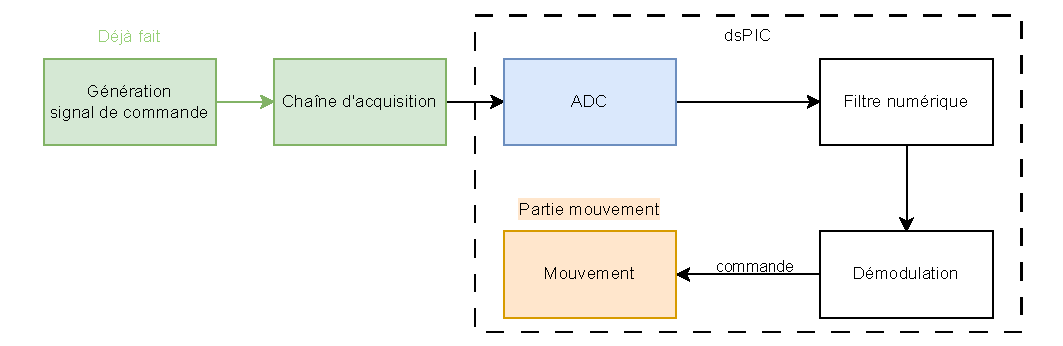
\includegraphics[scale=0.8]{pdffiles/ADCbloc.drawio.pdf}
    \caption{Schéma-bloc de la partie communication, focus sur l'ADC}
    \label{fig:adcbloc}
\end{figure}

Tout d'abord, nous devons configurer le périphérique du dsPIC chargé de la conversion à l'aide d'une librairie. Celle-ci inclut deux modes de fonctionnement :

\begin{itemize}
    \item [$\bullet$] \textit{Manuel} : le déclenchement de la conversion est lancé par le code
    \item [$\bullet$] \textit{Automatique} : le déclenchement de la conversion est lancé par le débordement du \textbf{TIMER3}
\end{itemize}

C'est ce deuxième mode qui sera utilisé car la démodulation est un processus qui doit être rapide et le mode automatique se réalise sans l'intervention du CPU.

Après avoir configuré le périphérique, on doit fixer la période d'échantillonnage de l'ADC en fixant la période de débordement du \textbf{TIMER3}. Mais avant, il faut déterminer cette période d'échantillonnage.

La fréquence d'échantillonnage est choisie telle que les fréquences qui se replient sur les fréquences utiles soient atténuées. Cela revient à choisir, au minimum, 2 fois la fréquence au milieu du segment formé par la fréquence de coupure du filtre de garde et la première fréquence atténuée par le filtre de garde (atténuation à 0.05). Ceci est représenté sur la figure \ref{fig:fs}.  

\begin{figure}[H]
    \centering
    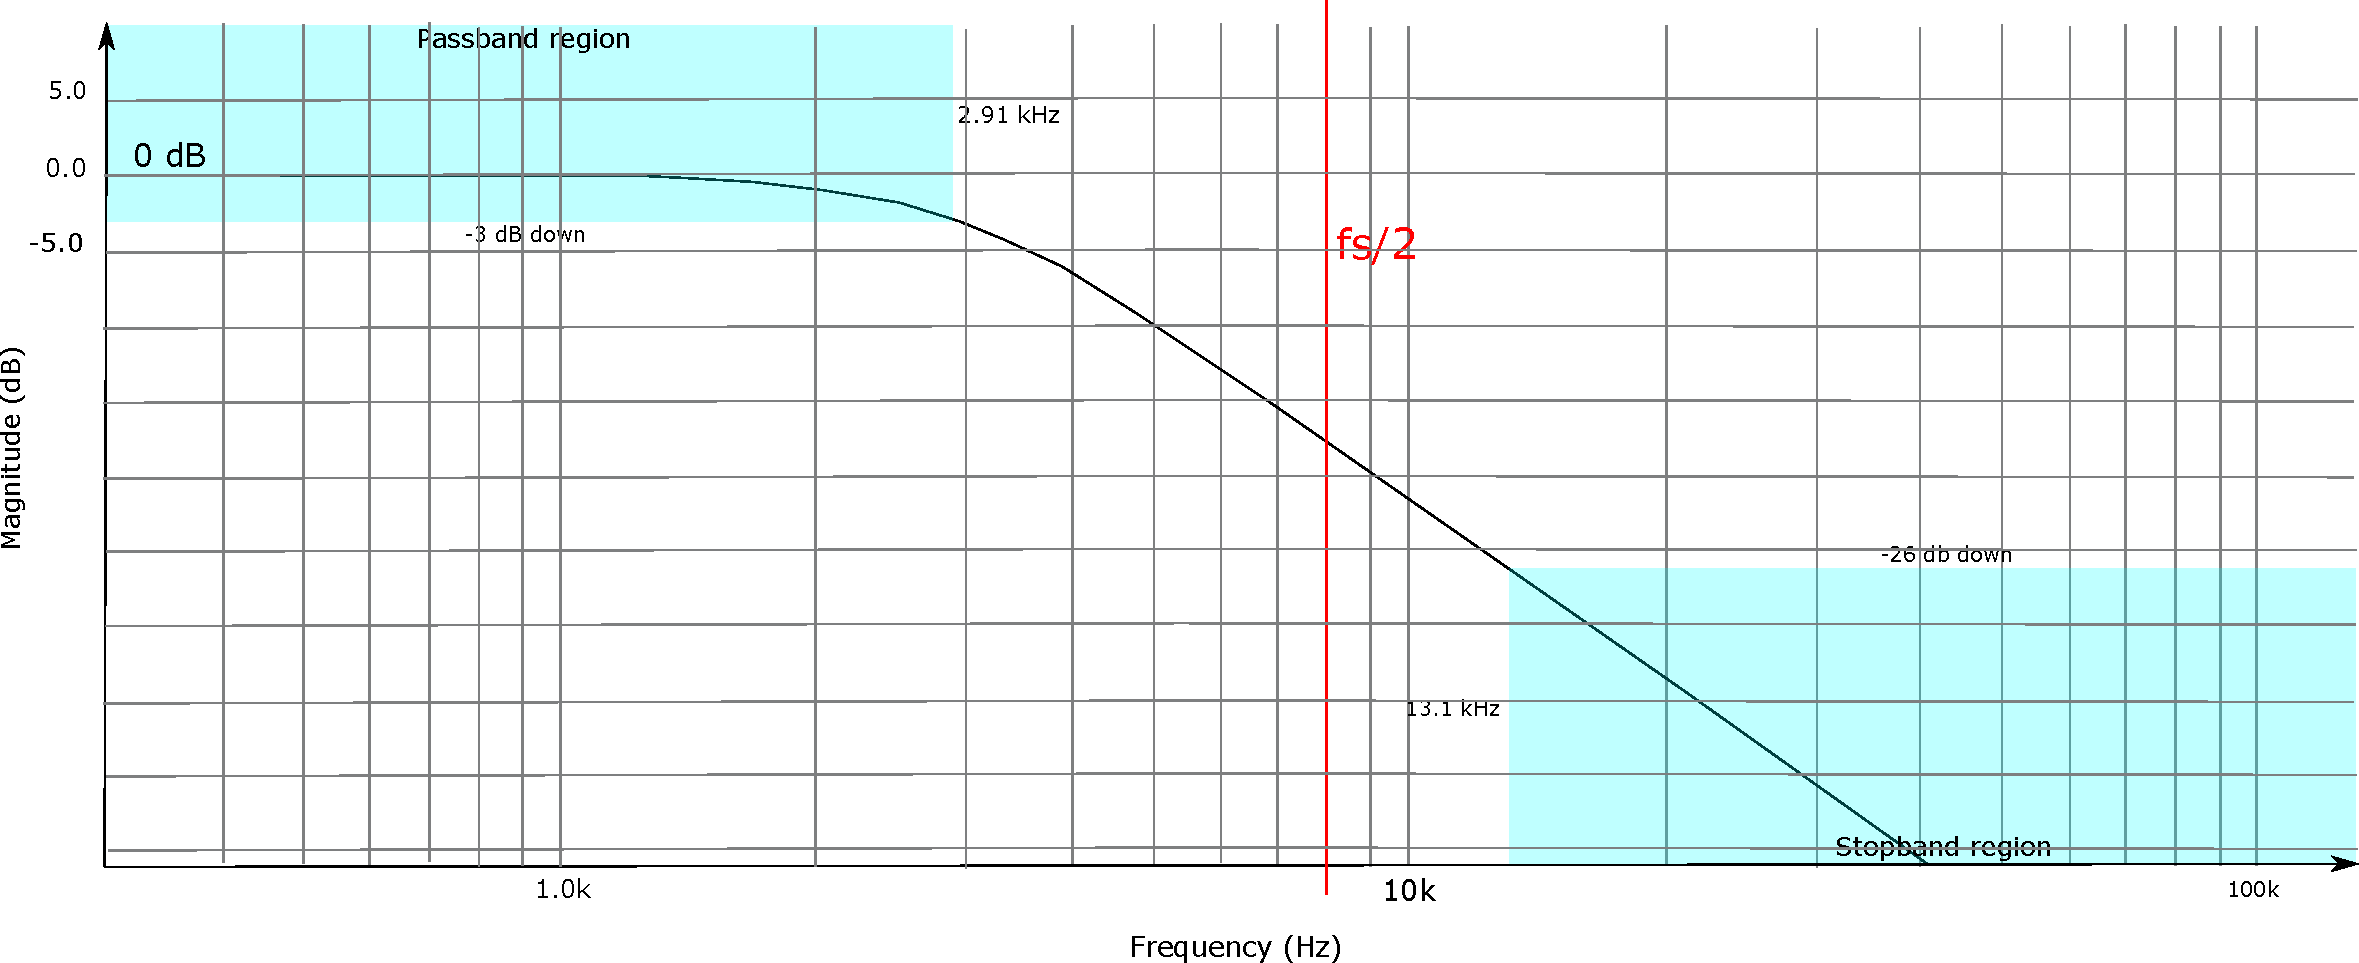
\includegraphics[width=1\textwidth]{pdffiles/lowpassspecINK.pdf}
    \caption{Illustration de la fréquence d'échantillonnage sur la courbe de Bode du filtre de garde}
    \label{fig:fs}
\end{figure}


Autrement dit, la fréquence d'échantillonnage minimale vaut :

\begin{align*}
    f_s &=\left(f_c+ \frac{f_{\text{repliement}}-f_c}{2}\right) \times 2 \\
    &= f_c + f_{\text{repliement}} \\
    &= 2914.050095+13023.87554 \\
    &= 15937.92545 \ Hz
\end{align*}

On peut à présent déterminer la période de débordement à partir de la formule suivante\footnote{On peut remarquer que FCY vaut 40 MHz : on a overclock le dsPIC} :

\begin{align*}
    & PR3 = (FCY \times T_s) - 1 \\
    & \text{Sachant que $FCY$ vaut $40 \ MHz$ et que $\frac{1}{f_s}=62.7434 \ \mu s$,} \\
   \iff & PR3=(40 \ MHz \times 62.7434 \ \mu s) -1 =2508.736 \\
   \hookrightarrow & PR3 \approx 2508 
\end{align*}

On arrondi PR3 à l'entier le plus bas, de cette façon la fréquence d'échantillonnage est plus grande que la fréquence minimale.

Il ne reste plus qu'à implémenter le code dans le dsPIC. On peut tout simplement reprendre le projet adc-dac2.X disponible dans le gitlab du projet et le modifier un peu.

\subsubsection{Validation de l'ADC}

Avant de passer à la démodulation du signal de commande audio, il faut vérifier que l'ADC fonctionne correctement. Pour vérifier que le signal numérique correspond au signal d'entrée, on peut utiliser le projet oscilloscope.X. En effet, en reliant le dsPIC à un PC à l'aide d'un périphérique UART $\leftrightarrow$ USB, on peut observer la forme du signal numérisé. 

Après avoir modifier le nombre de samples et la période d'échantillonnage dans le fichier oscilloscope.py, on peut afficher le résultat de la conversion. Les figures \ref{fig:900HZADC} \& \ref{fig:1100HZADC} nous permettent de valider le bon fonctionnement de l'ADC.



\begin{figure}[H]
    \centering
    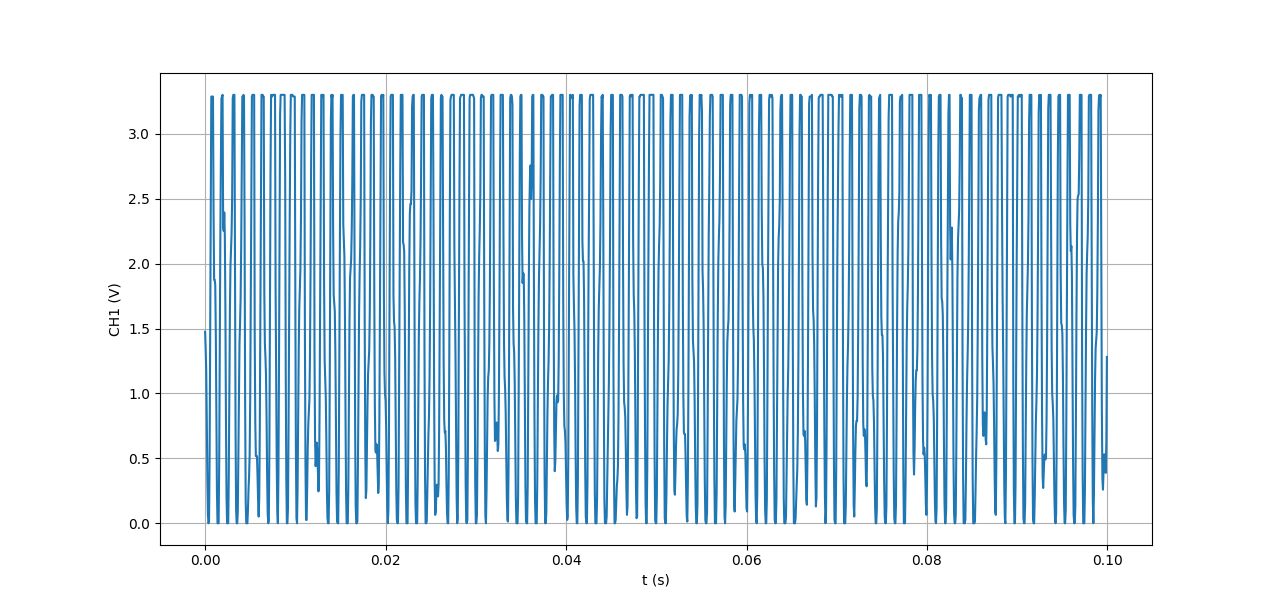
\includegraphics[width=0.7\textwidth]{Pictures/900HZ_ADC.png}
    \caption{Signal numérisé par le dsPIC. Le signal d'entrée est un signal audio de 900 Hz}
    \label{fig:900HZADC}
\end{figure}

\begin{figure}[H]
    \centering
    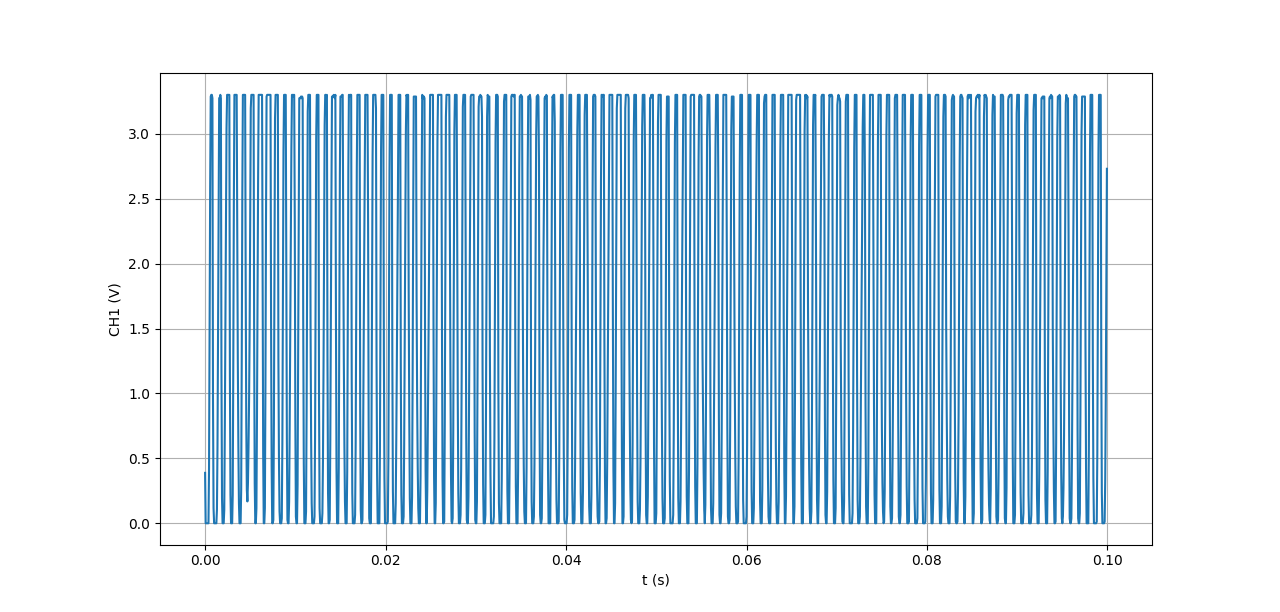
\includegraphics[width=0.7\textwidth]{Pictures/1100HZ_ADC.png}
    \caption{Signal numérisé par le dsPIC. Le signal d'entrée est un signal audio de 1100 Hz}
    \label{fig:1100HZADC}
\end{figure}

\textbf{Remarque} : Il faut modifier la manière dont les données sont envoyés via l'UART. On ne peut pas directement envoyer le résultat d'une conversion via l'UART car le temps que la donnée s'envoie, le \textbf{TIMER3} déborde et on perd de l'information. Il y a deux manières de régler ce problème.

\begin{itemize}
    \item [$\bullet$] Augmenter le débit de la transmission UART
    \item [$\bullet$] Attendre la fin de l'acquisition pour envoyer les résultats à l'ordinateur
\end{itemize}

Nous avons opté pour la deuxième solution dans le cadre de la validation de l'ADC.